\section{Welcome to the Black!}

\begin{multicols}{2}
  The year is 3210 and the Black is just waiting to be explored... again. Intelligent alien species (including humanity, I guess) once explored, expanded, exploited (and even exterminated) their way across the stars. That is until a sudden cosmic event known as \textbf{The Surge} threw everyone back into the stone ages.

  But we have (mostly) persevered in the face of adversity, and we stand on the shoulders of our ancestors to rebuild what we have lost. We have (kinda) rediscovered space flight, artificial intelligence, genetic modification, and terraforming. The Black is once again an empty canvas, waiting for us to paint civilisation all over it once again.
  
  \subsection{A brief history}

  Humanity, despite the set-backs, took their first steps into the Black back around the 1970's. We somehow managed to escape ancient Earth using only simple "propulsion thrusters" (engines that spewed matter out from one end to create movement in the other direction). It took about another century (humanity always was a late bloomer) to explore their local star system, and a further century to figure out how to terraform and colonise it. During that time they also figured out how to do \textit{real} artificial intelligence, put computers inside our brains, make deadly energy weapons, and all sorts of other cool technology.

  But the game-changer came with the invention of the \textbf{Trans-Dimensional Drive} during the 2200's, commonly known as TDD. This special machine allowed us to bend the laws of Space-Time for Faster Than Light (FTL) travel using what the tech-heads call "\textbf{trans-dimensional energy}". The TDD allowed us simple apes to escape the local star system and \textit{really} explore the big ol' Black.

  As it turned out, sentient life was common enough in the galaxy and TDD was the main form of FTL travel. We soon made first contact with dozens of alien neighbours and created some new friends (we \textit{may} have nuked a couple of others... but trust me, they were probably nasty). The friendlier aliens had already formed some sort of "federation of planets", and humanity entered the brutal arena of galactic politics.
  
  We eventually learned about the side-effects of TDD tech on organic beings. It just so happens that you begin experience changes when you are exposed to trans-dimensional energy. Some develop the ability to manipulate Space-Time, but most are just driven mad. The lucky ones became known as psionics, psychics, paranorms, or jsingshen. The federation created dedicated research centres to study and train psionics so that they could be a carefully controlled asset to civilisation.
  
  We colonised new star sectors and linked everything together using gigantic \textbf{TDD Jump Portals} that allowed us to instantaneously travel across our empire. We created technological marvels, cracked cosmic puzzles, tamed toxic landscapes and even expanded the limits of conciousness. The Black fell to civilisation's insatiable curiousity.

  And then it all came crashing down.
  
  \vspace{\baselineskip}

  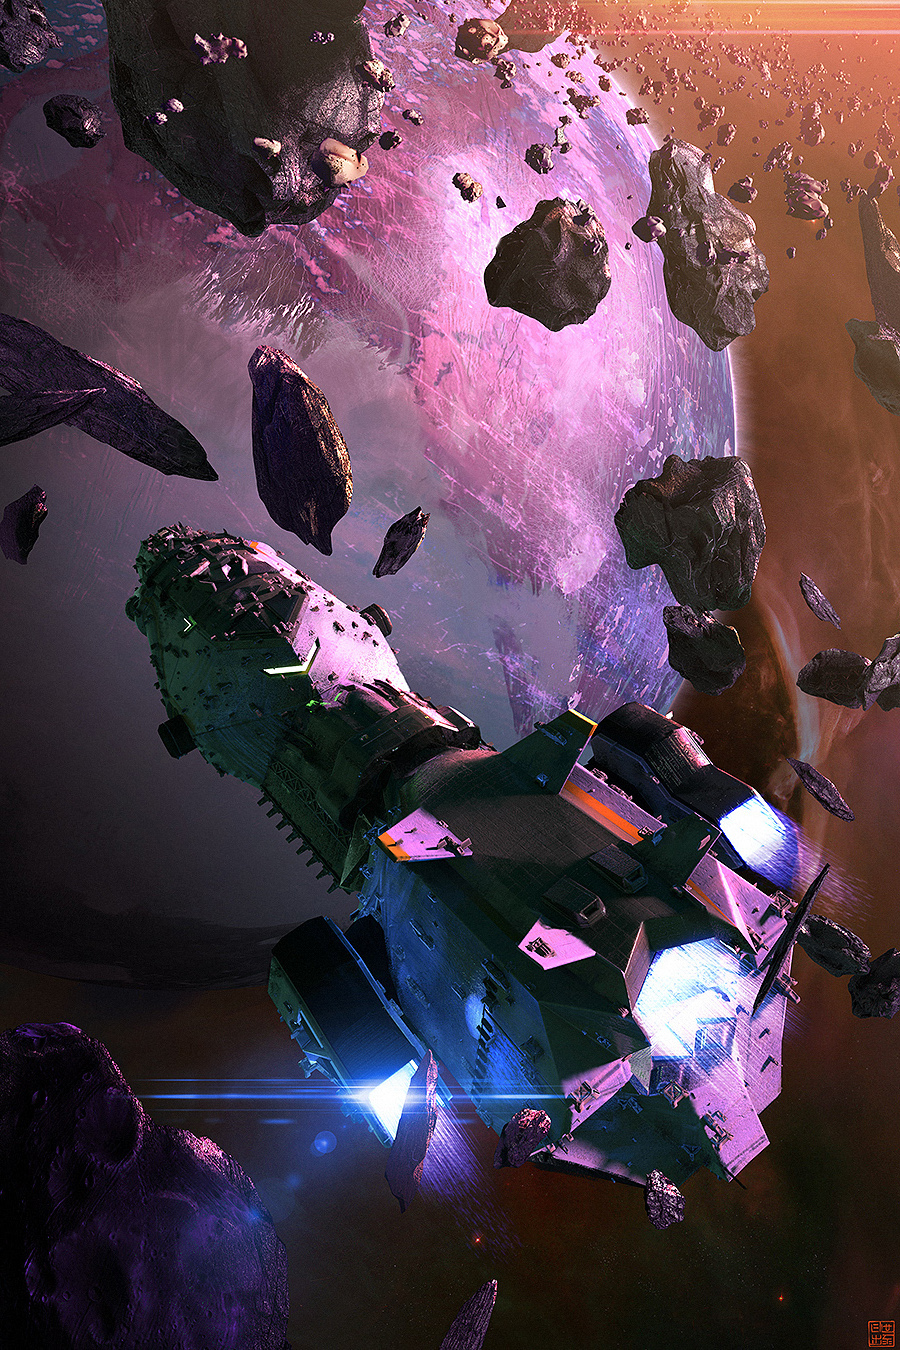
\includegraphics[width=\linewidth]{rebellion_of_stars___starship_blackbeard_by_hideyoshi-d8p607x}
  
  \subsection{The Surge}

  We call it \textbf{The Surge}, but very little is actually known about the event. Most tech-heads think it was a large shockwave of trans-dimensional energy that exploded from deep within the galactic center around about the 2800's, which simply overloaded all of our TDD tech. In a matter of seconds everyone lost their Jump Portals, TDD engines and even psionics to The Surge.

  The aftermath was terrible. Many worlds began to starve as they relied on the food imports delivered to them by the extensive FTL trade network. Other worlds slid into barbarism as they fought over now dwindling resources. All across the Black, countless worlds began their struggle due to their sudden isolation.
  
  It was even worse for the psionics. All the adult psionics suffered literal brain explosions during The Surge, leaving behind only the children (no one knows why they were spared). The children had to learn to safely harness their powers without the guidance of experienced mentors. To make it worse, they had to endure the fear and loathing of other survivors as rumours spread that The Surge was psionic handiwork.
  
  \subsection{Rebuilding the Galaxy}

  Over the last few centuries we have managed to rebuild. It isn't quite like the old days, but we are slowly piecing it back together. The one saving grace was that non-TDD tech was spared. Many planets filled the gaps left by the defunct TDD tech by adapting this so-called "outdated" tech. Some planets even refuse to advance further in fear that another Surge event could suddenly destroy all that they have built.
  
  In 3120, the Kaj tech-head Romazirash reverse engineered a safer (well, as it claimed) derivative of the TDD engine. It is called the \textbf{Intra-Dimensional Drive (IDD)}, and while it cannot travel across the whole galaxy it can travel across multiple star systems. The new IDD drive has allowed trade routes to be restored, and fledging federations of system begin to carve out their small sections of galaxy to govern. 
  
  Civilisation once again turns it's hungry eyes towards the edges of the Black. Warlords and petty tyrants scheme to expand their stellar domain. Reclaimers plunder the ruins of worlds that did not survive. And psionics continue to practice their skills away from the distrustful eyes of those who see the use of trans-dimensional energy as an imminent threat to their way of life.

  \textbf{Good luck out in the Black!}
  
  \textit{P.S: Remember: It's dangerous to go alone! Take friends.}
\end{multicols}

\vspace{\baselineskip}

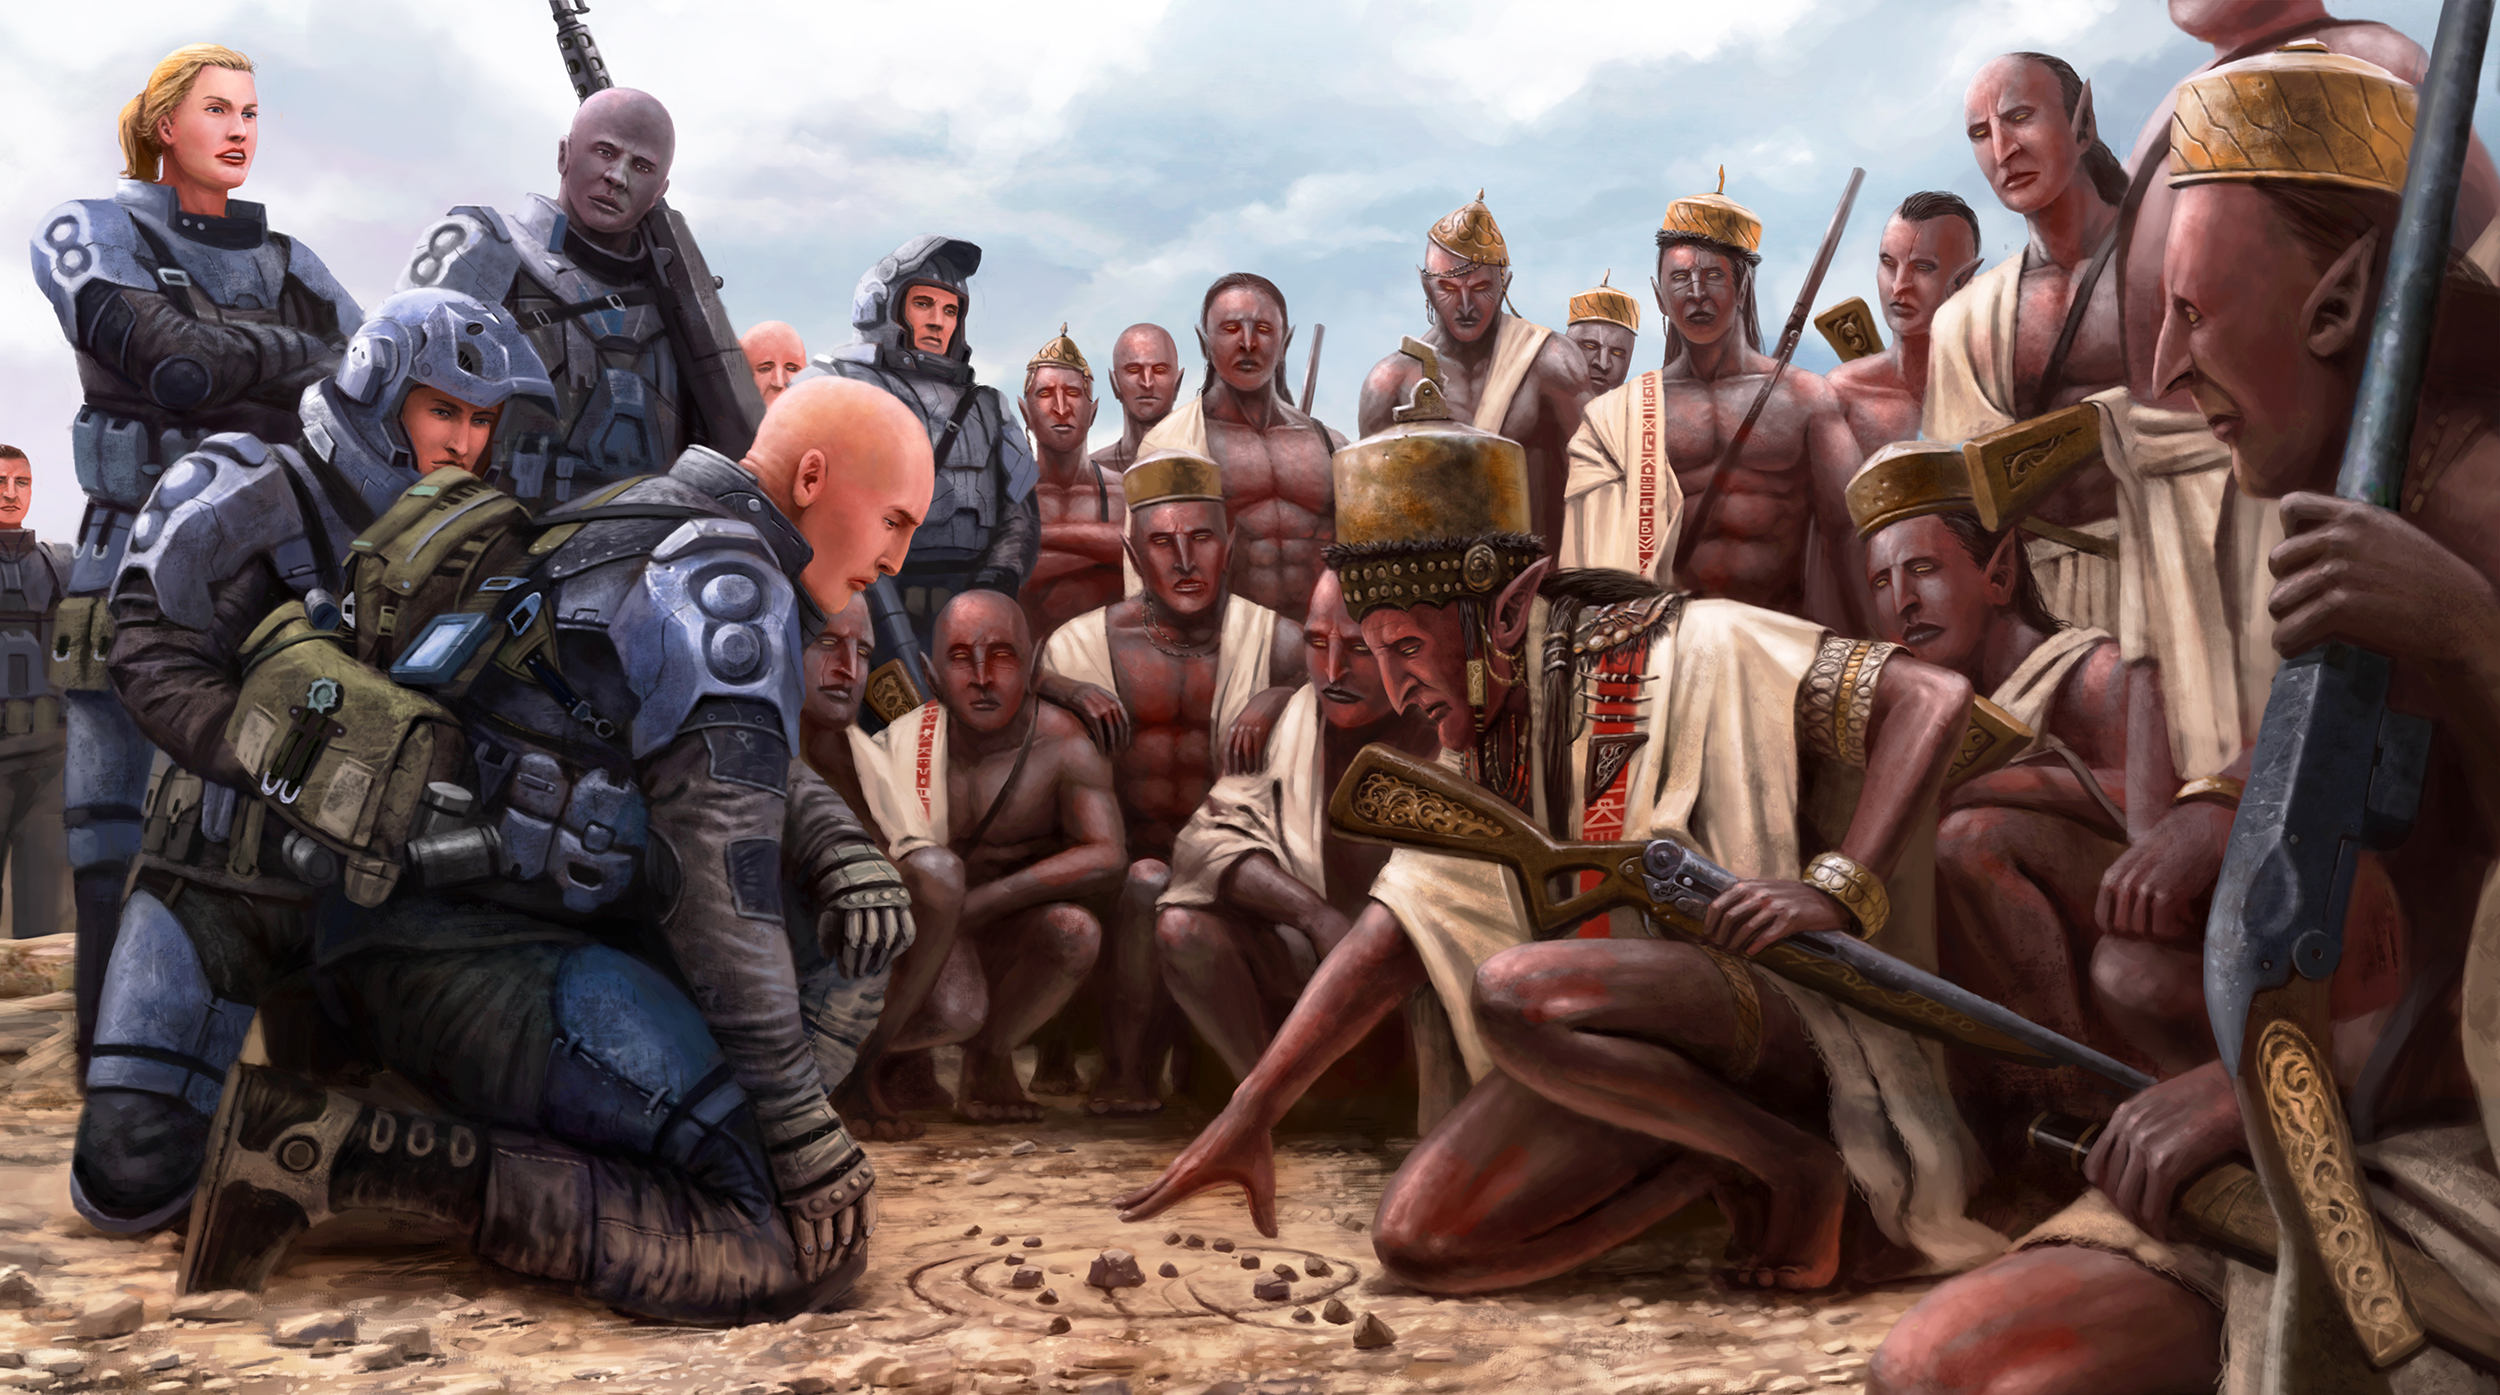
\includegraphics[width=\linewidth]{joint_operation_by_skaya3000-d6styjt}
